\documentclass[titlepage, 12pt]{article}
\usepackage[utf8]{inputenc}
\usepackage{comment}
\usepackage{a4wide}
\usepackage{hyperref}
\usepackage{graphicx}
\usepackage{caption}
\usepackage{subcaption}
\usepackage{float}
\usepackage{setspace}
\usepackage{epstopdf}

\onehalfspacing

\graphicspath{{./figures/}}

\title{Evolution of sex in Artificial Life using NEAT \\ \large Natural Computing Project Report}
\author{Jules Kruijswijk \\ s4140023 \and Paul Bertens \\ s4512448}
\date{\today}

\begin{document}

\maketitle

\tableofcontents

\newpage

\begin{abstract}
In the vast area of theories on evolution of sex, there are a few interesting theories which touch on the advantages of sexual reproduction over asexual reproduction.
However, it still remains a question why sexual reproduction is as common as it is in the natural world.
Using digital life simulations in Avida, it was found that sexual reproduction is more advantageous in rapid changing environments (a rapid changing environment is an environment where nutrient and poisonous food are swapped, where poison becomes nutrient food and vice versa).
In this report we try to extend this hypothesis to a more ecologically valid situation, but with the same question and hypothesis.
Our research question is if sexual reproduction is more advantageous in a fast changing environment than in a static environment in the used simulation.
An Artificial Life simulation was developed where the agents had neural networks as brains.
The neural networks were evolved using the NeuroEvolution of Augment Topologies (NEAT) algorithm, which evolves the neural networks in their topologies and the assessed weights.
The environment that was created consisted of poisonous and nutrient food, which, as their names suggests, either reduce or increase the energy of an agent.
The experiment consisted of two conditions, one condition where the environment was kept static (thus the food did not swap) and the second condition where the environment was dynamic.
The results showed that the amount of sexual reproduction (measured in average crossover per run, with a total of 30 runs per condition) is significantly more in the dynamic condition than in the static condition ($p = 0.00006335$).
Various ways to investigate the findings and improve the results are highlighted in the discussion section.
\end{abstract}

\section{Introduction}

There are many theories on the evolution of sex and on the advantages of sexual reproduction over asexual reproduction \cite{misevic, michod1988evolution}. 
It remains an open question as to why sexual reproduction is so common in the natural world despite the relatively higher cost over asexual reproduction. 
The paper by Dusan Misevic et al. \cite{misevicchanging} tests the hypothesis that sexual reproduction is advantageous in changing environments using digital organisms. 
The digital organisms were simulated in Avida, in which the organisms are short self-replicating computer programs. 
They then modified the metabolic values of poisons and nutrients such that they could switch and change in value. 
They found that sex became the dominant mode of reproduction when the environmental change was rapid and substantial enough. 
Thus the study finds support for the importance of changing environments in the evolution of sex. 

\subsection{Theories of Evolution}

The review paper by Matthew hartfield and Peter D. Keightley \cite{matthewhartfield} gives an overview of some of the dominant theories on the evolution of sex. 
The four classes of theories discussed are: The Fisher-Muller hypothesis, Muller's ratchet, Red Queen hypothesis and the mutational deterministic hypothesis.
The Fisher-Muller hypothesis states that sexual reproduction allows natural selection to work faster than when reproducing asexually since recombination can bring together advantageous genes faster than asexual reproduction could.
Muller's ratchet states that sex evolved to fix multiple advantageous mutants as a mechanism to stop the build-up of deleterious mutations in finite populations. 
In asexual reproduction bad genes can build up, known as genetic load, which would lead to an organism going extinct. 
Sexual reproduction could counter this by recombination, stopping the build-up of these bad genes.
The Red Queen hypothesis is the hypothesis that sexual reproduction evolved due to co-evolution of opposing organisms in a rapidly changing environment. 
Sex allows for faster adaptation to these changing environments and gives a higher chance of survival.
Mutational deterministic hypothesis assumes that the majority of deleterious genes are only slightly bad, but that each additional bad gene increasingly reduces the fitness of the organism. 
Sexual reproduction will generate offspring with fewer deleterious genes and some with more, those that have more will quickly die out but those with few will survive. 
Thus sex can help remove these slightly deleterious genes that only combined have a large effect.
They conclude that theoretical and experimental results favor the hypothesis that sex allows for the recombination of advantageous genes (The Fisher-Muller hypothesis), or acts as a mechanism to shuffle genotypes in order to repel parasitic invasion (Red Queen hypothesis) which is in line with our main hypothesis.

\subsection{Research Question}

One hypothesis, as stated before, is that sexual reproduction does better in a faster changing environment \cite{misevicchanging}. 
One explanation for this is that sexual reproduction allows for faster adaptation in a fast changing environment due to recombination. 
With recombination groups of genes can be swapped faster which would result in higher variations and a higher chance of adapting to the new environment.
The study however is not very ecologically valid, since it performs on logical operations and its environment does not match the real world. 
We therefore will use NEAT \cite{stanleyneat}, an evolutionary algorithm which operates on neural networks, in a simulated environment. 
The proposed research question is as follows.
Is sexual reproduction more advantageous in a fast changing environment than in a static environment?
Although the simulation is a gross simplification it is still closer to the real world than Avida and should give better insight into the advantages of sexual over asexual reproduction.
To investigate this issue, we will develop a simulation in Java, which will have the same or more parameters than the Avida simulation software.
Based on earlier research and the fact that the proposed environment is an even better suit for simulations, we hypothesize that sexual reproduction is more advantageous in a faster changing environment than in a static environment.


\section{Methods}

To see whether sexual reproduction is indeed preferred over asexual reproduction in a fast changing environment, an Artificial Life simulation was designed in Java. In this simulation, NEAT was used as an algorithm to evolve recurrent neural networks, which will be the brains of the agents.

\subsection{Simulation}

The simulated world is a simple 2D world with both food and poison represented by different colors.
In the environment, the agents will move around and eat food to collect energy.
The simulation is completely written in Java\footnote{For source code, see \url{http://github.com/g0ulash/NEATSimulation } NOTE: THIS GitHuB IS STILL PRIVATE}.

\subsubsection{Environment and Parameters}

The environment consists of an empty field where food and poison are randomly spawned away from other food and agents - see Figure \ref{fig:env} for an example.
The environmental changes will be the food and poison, which will have some chance of switching and changing in value resulting in food becoming poison and vice versa. 
Obviously, nutrient food gives agents energy and poisonous food reduces the energy of an agent.
The amount of food will always be kept constant, so if one piece disappears there will be a new spawned piece of food on a random place.
There are also the borders, which enclose the environment.
If an agent collides with the border it will also lose energy.

\begin{figure}[H]
\centering
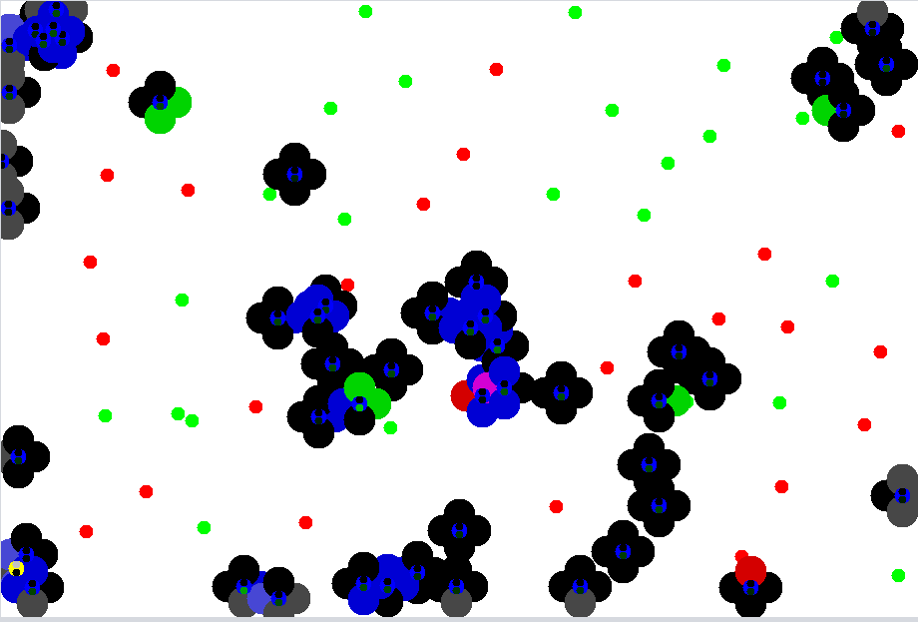
\includegraphics[scale=0.5]{environment.png}
\caption{An environment filled with agents, poisonous and nutricious food.}
\label{fig:env}
\end{figure}

\subsubsection{Agents}

Each agent, see Figure \ref{fig:agent} for an example, will have a recurrent neural network as a brain, which will be evolved using the NEAT algorithm.
They will inhabit this environment and have an extra evolvable parameter that determines whether they will reproduce sexually or asexually. 
The age of the agents is the number of iterations that it has been alive, which will also be the fitness function.
Each iteration, agents lose energy and when their energy is fully depleted, they will die.
So their goal is to try and find nutrient food and avoid poison to replenish their energy.
If they reproduce asexually they can only create offspring with mutation, while if they reproduce sexually they can create offspring with cross-over and mutation. 

The input to the neural network of each agent are four color sensors for each direction that can read the pixel value next to them.
Each color sensor is an RGB valued sensor, which results in $12$ input represented as floats.
The last two inputs will be their own energy level and a bias input, which makes it a total of $14$ inputs.
The output will be their movement which are output as 2 dimensional coordinates.
The activation function of the neural network is a hyperbolic tangent so that the output is between $-1$ and $1$ for both of the directions. 

\begin{figure}[H]
\begin{subfigure}[b]{0.5\linewidth}
    \centering
    
\includegraphics{agent_nofood.png}
\end{subfigure}%
\begin{subfigure}[b]{0.5\linewidth}
    \centering
    
\includegraphics{agent_food.png}
\end{subfigure}
\caption{Agents as represented in the simulation. The left agent is an agent in rest state, which has nothing surrounding to sense and the right agent is one that senses food.}
\label{fig:agent}
\end{figure}

\subsubsection{Updates}

The number of the agents in the environment is kept constant.
For example, if two agents die then two new offsprings are created using NEAT.
The agents that will be selected using roulette wheel selection, where the probability of selecting an agent is proportional to his fitness function, which is the age of an agent.
Thus if an agent is older, it has a higher probability of being selected.

\subsubsection{Parameters}

The parameters that can be set in the environment are as follows. 
The amount of food and poison and the number of agents can be set.
Agents start with a set, by the user, starting energy.
There are certain parameters which concern the energy loss or bonus for specific scenarios.
One of them is the energy bonus and loss for eating food and poison respectively.
An energy loss can also be set for when an agent hits the border and for the crossover and mutation.
Then also each update an energy loss will be calculated based on the brain size cost ($\frac{(\#nodes+\#connections)^2}{c}$, where $c$ is the parameter to be chosen).
There is a parameter to set after how many iterations the poison and food will switch.
A mutation rate can be set for both nodes and links (after the explanation of NEAT it will become clear what nodes and links do).
And lastly there is a mutation rate for sexuality, which means that an asexual agent can become sexual and vice versa.

\subsection{NEAT}

To implement the NEAT algorithm, we will refer to the original paper \cite{stanleyneat}.
Modeling and evolving Artificial Neural Networks (ANNs) in a genetic algorithm is not trivial, because the structure of different neural networks are not necessarily related.
To perform crossover operations, the network structures have to be analyzed to find appropriate crossover points, and naturally the genomic representations for ANNs do not clearly show where these points are.
With NEAT the authors have tried to overcome this problem by encoding history in each element of every single genome.
This guarantees that structures are identifiable and thus analyzed more easily.

Each genome in the algorithm consists of a list of nodes and a list of connections.
Each connection has values for its input node, output node, the weight on the connection, whether the link is enabled or not and a so called innovation number.
The innovation number is the historical value, which allows the crossover operations to detect if the gene is similar to another gene in a different genome.
Each node contains a unique identification number, whether it is enabled or not and also an innovation number.

\begin{figure}[H]
\centering
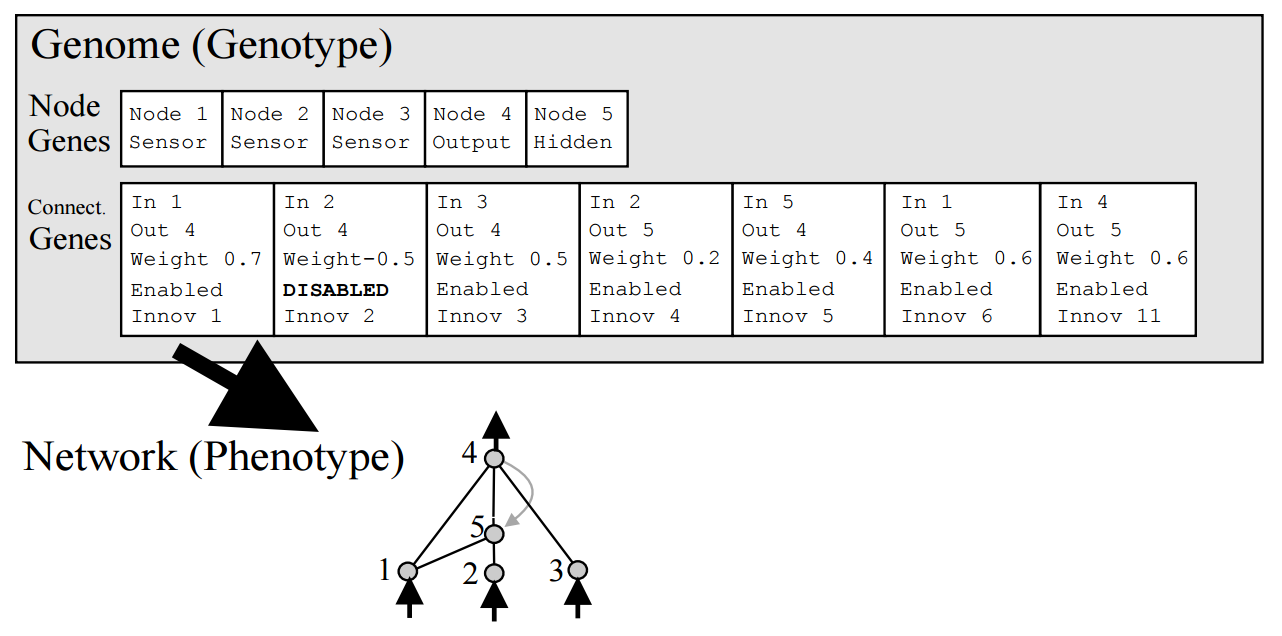
\includegraphics[width=\textwidth]{genopheno.png}
\caption{Genotype to phenotype mapping in NEAT.}
\label{fig:gen}
\end{figure}

Mutation can occur randomly in NEAT and it can change connection weights, activation thresholds and the network topology.
The weights and thresholds can be changed when a random connection or node is chosen and the values are constrained.
The network topology changes by randomly adding nodes or connections.
When an connection mutation occurs, the algorithm first randomly selects two nodes.
If there did not exist an connection yet, it will then insert an connection with initial weight one.
If an connection already existed, the only thing it will do is enable the connection again if it was disabled.
And a last special case, if there is no connection between the two nodes, but an equivalent connection is already present in another genome of the population, this connection will be copied with the same innovation number - the reason for this is that it is not a new innovation.
Mutation of nodes arrives in another fashion, as instead of randomly choosing two nodes, the algorithm now takes an connection, disables it and also adds a new node.
This node, with a random activation threshold, will be connected to the nodes that were connected to the disabled connection - effectively creating two new connections as well.
The weight of the disabled connection will be copied to the output connection of the new node and the weight of the input connection will be set to one, such that it does not interfere with any learning that has taken place, yet.

\begin{figure}[H]
\centering
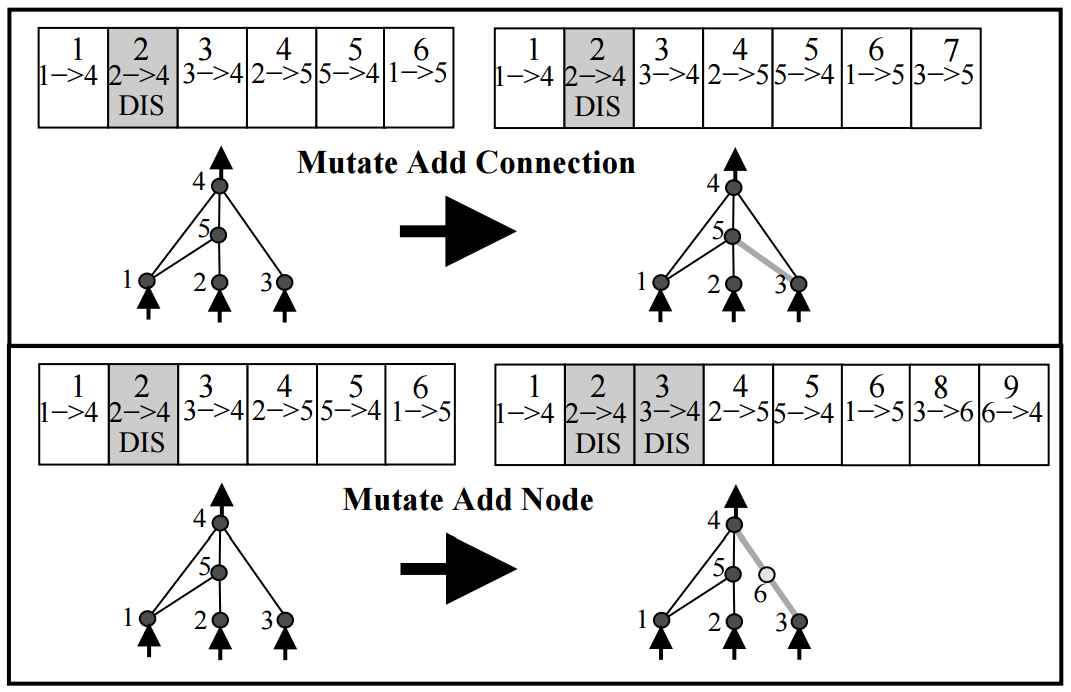
\includegraphics[width=\textwidth]{mutation.png}
\caption{The two types of mutation in NEAT.}
\label{fig:mut}
\end{figure}

Before crossover can be introduced, the innovation numbers have to be explained.
Since the innovation numbers are not unique to genes specifically but only to the innovation (i.e. new gene), you can compare two genomes in the population and check if they share any genes.
If any of the genes share the same number, they also share the same manifestation. 
NEAT stores the innovations in a database that have occurred since the initial population.
Before a new innovation is introduced, the database will be checked if it does not already exist.
If it is a new innovation, the database will store the innovation and increment a global innovation number which will pass on to that gene.
This ensures that all related genes are eventually identical.

When a crossover operation is applied to two genomes, the new genome will receive the same innovation numbers in the genes.
Because NEAT uses these innovation numbers, it can easily align two genomes to see which parts are similar and which are different.
The genes that have different innovation numbers are called disjoint and added to the child during crossover.
Genes that have newer innovation numbers are called excess and also added to the child during crossover.
The genes that have shared innovation numbers are inherited by the parent genome that has the highest fitness value.
The crossover operations in this algorithm limit the support for big diversity, as a new innovation, which can have a high impact, can be erased from the population before it reaches its potential.

To overcome this problem, NEAT uses speciation.
In nature, speciation is defined as when two organisms once shared a genome sometimes diverge such that they can no longer mate with each other.
When a genome diverges far enough (according to a certain formula) from that of the other genomes in the population, NEAT will find this genome and put it in its own species.
It calculates the distance based on the excess and disjoint genes and the average weight differences of two genomes - each of these parameters are weighted.
The initial population consists of one species.
Following new generations, NEAT can identify a genome that should be in a new species and makes one accordingly.
If other genomes in one species are diverging from their own species towards another, the algorithm will transfer this genome between species.
Through certain fitness testing, NEAT can identify whether or not new genomes in a species have improved fitness compared to the original genome in that species.
If a species has not improved over a certain amount of generations, it can be deleted entirely from the population - because this means that a certain innovation did not have enough impact.
Based on the fitness value of the species, each species will have a percentage of spots for the new generation.
Due to time constraints, speciation was not implemented in the experiment.

\begin{figure}[H]
\centering
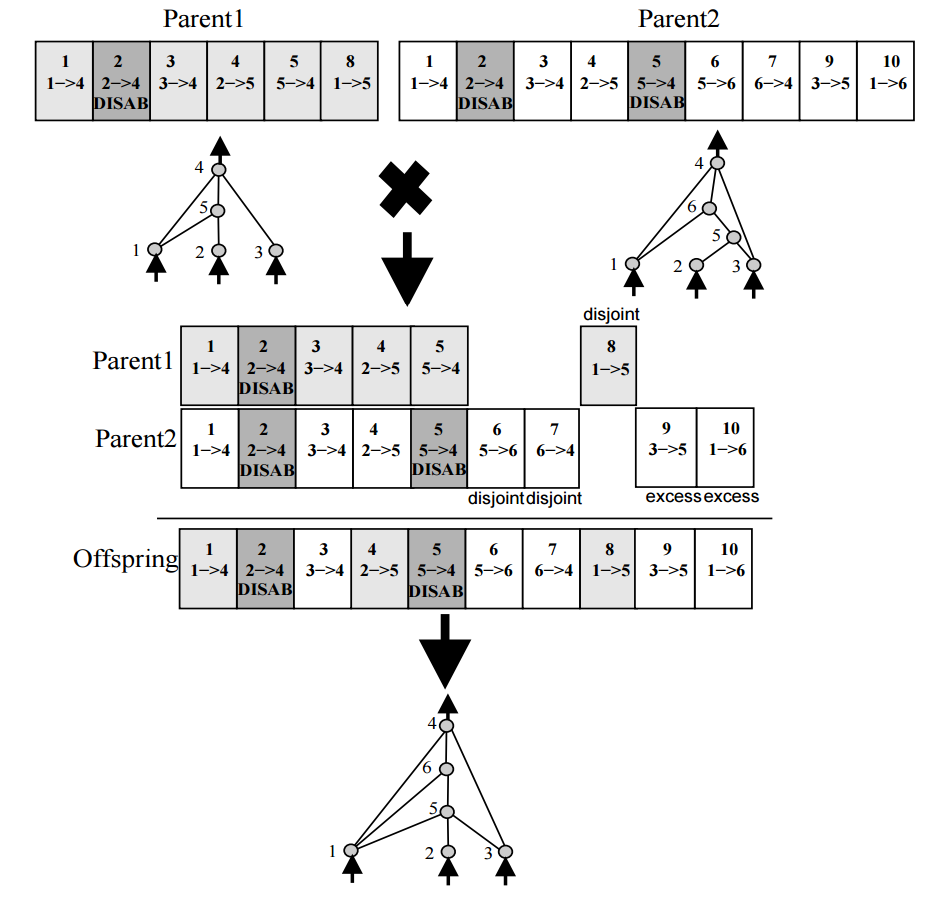
\includegraphics[width=\textwidth]{crossover.png}
\caption{Crossover as it is specified in NEAT.}
\label{fig:cross}
\end{figure}

\subsection{Experiment and Analysis}
In the experiment there were two conditions, a static and dynamic condition.
In the static condition means that the food will not switch between nutrient and poison, whereas in the dynamic condition this will happen after $2000$ iterations.
The number of agents and food was $50$ where poison and nutrient food were $25$ each.
The starting energy of the agents was $10,000$, the energy loss and bonus for food was $10,000$ for nutrients and poison respectively.
The constant for the brain size cost was set to $100,000$ and the energy loss when hitting a border was $2,500$.
The cost for crossover was $5,000$ and the mutation rates were $10\%$ and $1\%$ for links and nodes respectively.
The mutation rate for sexuality was $1\%$.

For each condition, $30$ runs were performed.
A few different type of results were obtained per run per $100$ iterations, namely the average fitnes, average age of the food, average age of the poison, number of agents, average fitness, average energy, average brainsize and average crossover.
To check for the hypothesis, the average crossover was tested for both conditions.
Other results such as the average fitness, average age of food et cetera will be shown to see what happened over time.
The parameters were the same for both conditions except for the switch of the food.
To test the data, first a normality test (specifically the Shapiro-Wilk test) was done after which the appropriate test was used.
If the data appeared to be normally distributed, a independent sample t-test were to be performed and a Wilcoxon rank-sum test (WRS) otherwise.
The condition (static and dynamic) is the independent variable and the average crossover is the dependent variable.
In the test the average crossover for each recorded iteration will be averaged to one average per run, which results in a test with $30$ samples per condition.

\section{Results}

Firstly, the main results that should answer the research question will be discussed.
After that, a few interesting insights that were gathered after the experiment will be shown.

\subsection{Main Results}
The mean for the static condition is $0.6051$ with a standard deviation of $0.2792$ and the mean for the dynamic condition is $0.8354$ with a standard deviation of $0.0872$.
Shapiro-Wilk test for both the static and dynamic data is not significant ($p = 0.0776$ and $p = 0.0592$ respectively), which means that an independent sample t-test can be performed. %when I have 6000 samples this becomes 0.1818 and 0.1192
The indepedent sample t-test showed that the data is significantly different ($p = 0.00006335$).
This means that the hypothesis that sexual reproduction is more advantageous than asexual reproduction in a faster changing environment can be accepted under this experiment.

\subsection{Descriptives}
To get a good insight in the data, it is interesting to see what happens over iterations, since properties such as average crossover, average fitness and age of food will change over time.
Figure \ref{fig:avgcross} shows the average crossover of the two different conditions over time.
The results that are shown are averaged over all $30$ runs.
The average crossover for the static condition declines slowly, but steadily over time.
It shows that although it has a high average of crossover, it keeps declining.
The average of crossover in the dynamic condition is quite steady, and apart from small fluctutations does not change.
Figure \ref{fig:avgfit} shows the average fitness (age of the agents) of the two different conditions over time.
It shows that in the static condition the average fitness increases to a high amount (up to $5,000$) and that it is very low in the dynamic condition (fluctuating around $200$).
Figure \ref{fig:avgfood} shows the average age of the food in both conditions.
The age of the food in the dynamic condition is the most prominent, since in the beginning it is relatively high and decreases over time (albeit with heavy fluctuations).
The age in the static condition stays very steady.
Figure \ref{fig:avgpois} shows the average age of the poison in both conditions.
In the static condition, the age increases by a large amount, whereas in the dynamic condition the age of the poison stays relatively low.
In the dynamic condition, the age of the food and the poison stay quite the same (around the $2,500$ lowering down to $1,000$).

\begin{figure}[H]
\centering
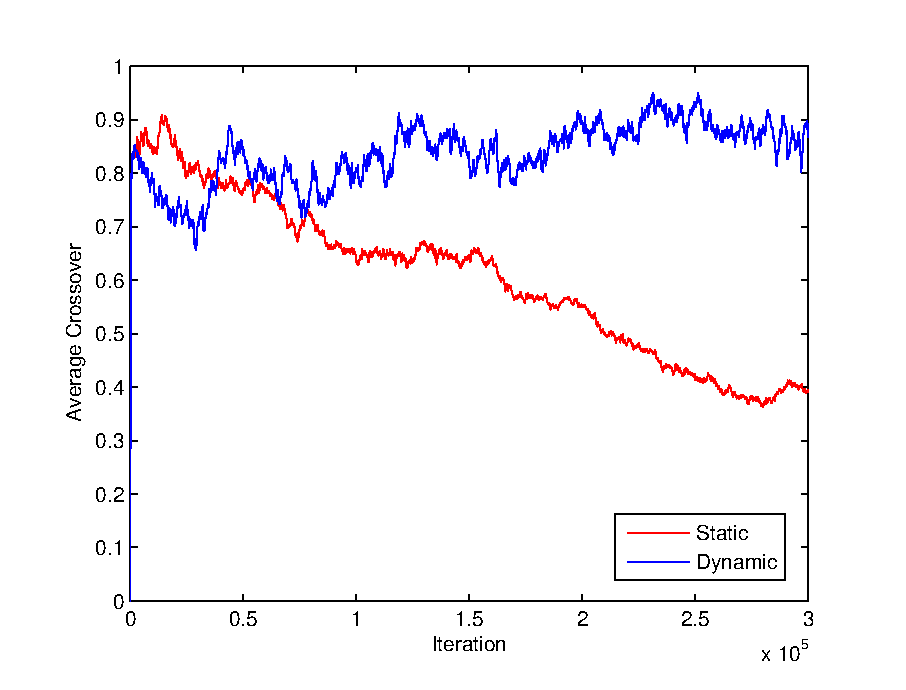
\includegraphics[width=0.75\textwidth]{average_crossover.eps}
\caption{Average crossover per condition. The results shown here are averaged over all $30$ runs.}
\label{fig:avgcross}
\end{figure}

\begin{figure}[H]
\centering
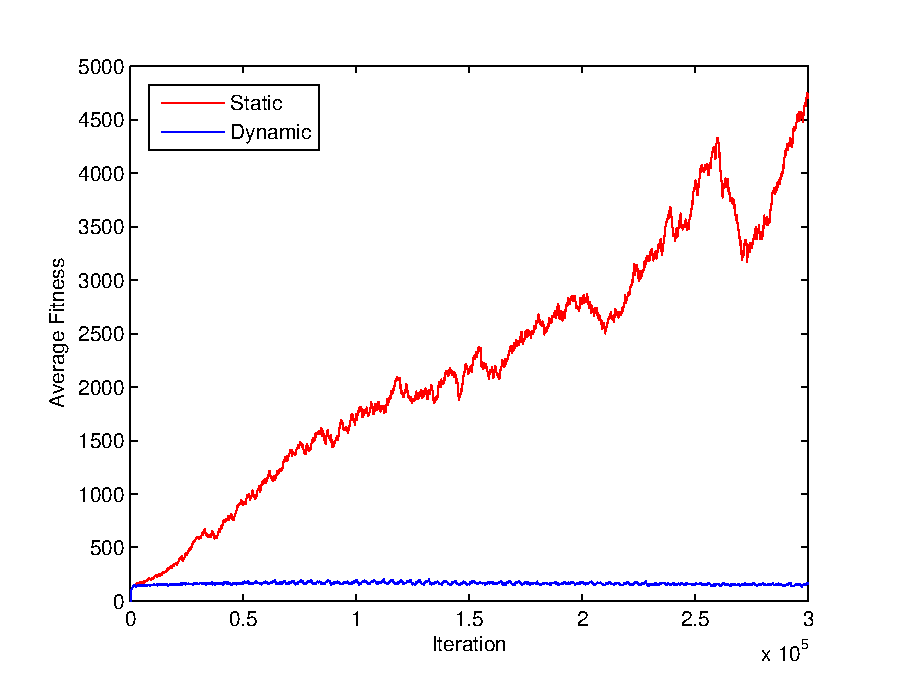
\includegraphics[width=0.75\textwidth]{average_fitness.eps}
\caption{Average fitness per condition. The results shown here are averaged over all $30$ runs.}
\label{fig:avgfit}
\end{figure}

\begin{figure}[H]
\centering
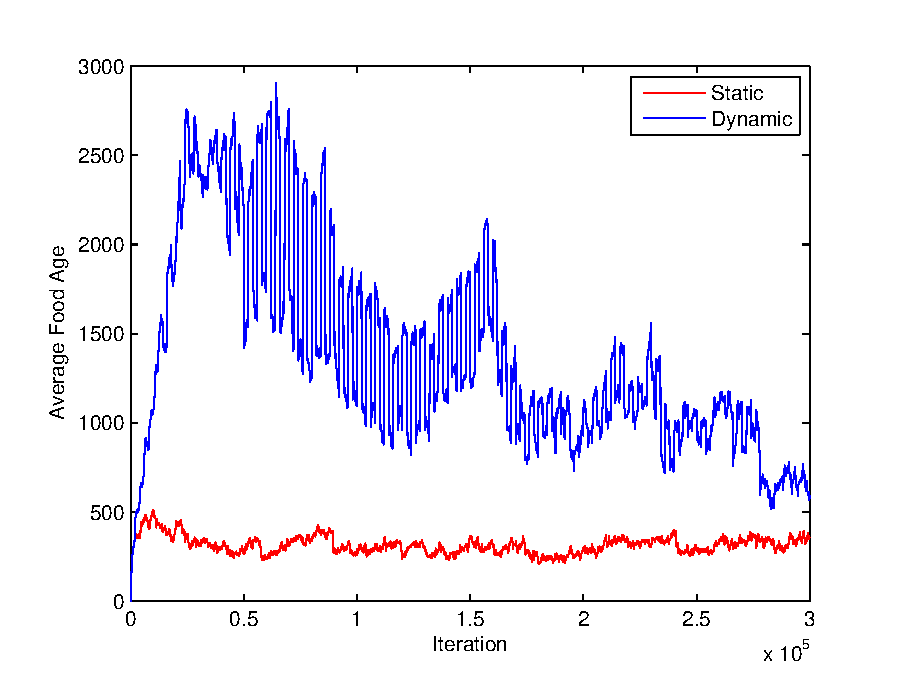
\includegraphics[width=0.75\textwidth]{average_food_age.eps}
\caption{Average age of food per condition. The results shown here are averaged over all $30$ runs.}
\label{fig:avgfood}
\end{figure}

\begin{figure}[H]
\centering
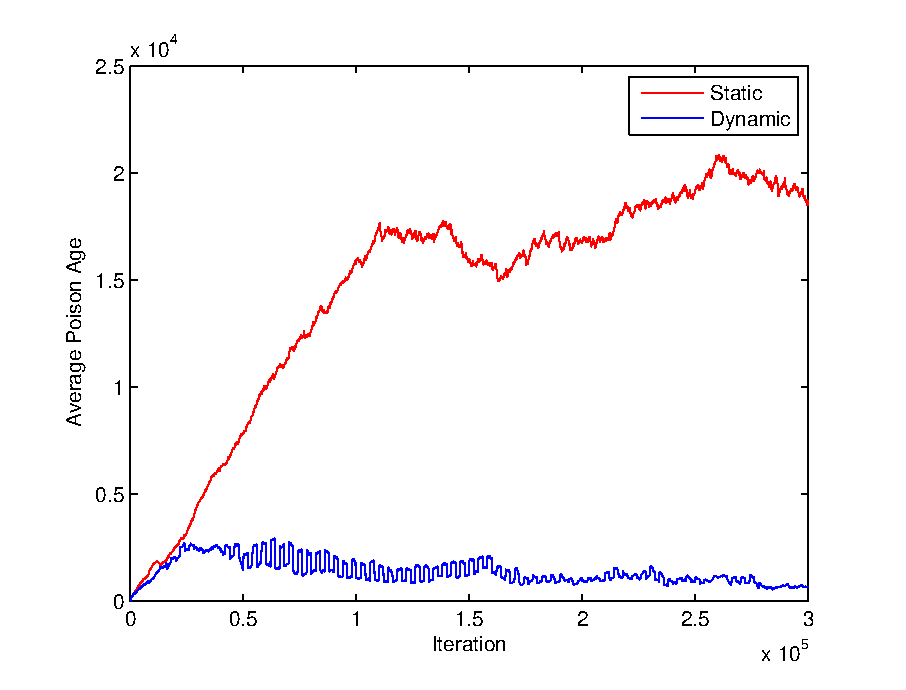
\includegraphics[width=0.75\textwidth]{average_poison_age.eps}
\caption{Average age of poison per condition. The results shown here are averaged over all $30$ runs.}
\label{fig:avgpois}
\end{figure}

\section{Discussion}

We found a significant difference between the average crossover in a dynamic environment and a static environment.
The results showed that sexual reproduction gets selected more in a dynamic environment than in a static environment.
This means that the findings that the earlier research had (i.e. in \cite{misevicchanging}) also extend to a more ecological valid simulation, using neural networks instead of the Avida simulation.
More extensive research where a more complex, more realistic environment could be interesting to find which influence sexual reproduction has on evolution.

Furthermore, looking at the descriptive results, a few interesting observations can be made.
Figure \ref{fig:avgcross} shows the average crossover of the two different (dynamic and static) conditions over time.
As explained in the results, the average crossover for the static condition declines slowly but steadily over time.
Now two observations can be made here, the first being that it would be interesting to see what happens to the average crossover when the simulation was run for more than the $300,000$ iterations that is has been run in this experiment.
If it keeps declining over time, it could show that eventually asexual reproduction is more advantageous in a static environment than sexual reproduction is - this should be tested with a different research question than in this experiment.
One of the reasons that potentially explain the decrease is that once the environment is known by the agents, i.e. they have learned their optimal solution, and there are no changes in the environment, the cost of sexual reproduction is too high to keep sustaining it compared to only asexual reproduction.
A new experiment that investigates the influence of the parameter such as crossover cost could point out in how far the cost of sexual reproduction is too high to sustain that type compared to asexual reproduction.
The second observation that can be made is that the declining of the average crossover perhaps can be influenced by the set parameters of the simulation.
An interesting experiment that could be looked at, would be to compare different dynamic conditions, where the food swaps are performed at different iterations, and see what influence it has on the average crossover rate and if it also shows a tendency to converge for other dynamic conditions.

Looking at Figure \ref{fig:avgfit}, it shows that the average fitness increases consistently in the static condition but stays at low values in the dynamic conditions.
Future research could investigate how to overcome this low fitness problem in the dynamic conditions.
The type of learning that is used in the simulation is something that can increase the average fitness.
In the case of the neural networks and the learning that is used right now, is that actually only the children of sexual reproduction can learn from this mistakes of their parents.
Perhaps combining the current experiment with reinforcement learning could allow the agents to learn from their mistakes more easily and eventually increase the fitness. %I am not sure if I put it correctly like this?

A final remark concerning the algorithm used in this experiment, is that future research could look into algorithms that are extensions of NEAT.
One of these algorithms is HyperNEAT, which shows a few interesting improvements compared to NEAT \cite{stanleyhypercube}.
HyperNEAT is able to evolve neural networks that look more like the neural and structural connectivity patterns as found in the brain, which enhances the validity of an Artificial Life - especially concering the ecological validitiy.
The second important feature that HyperNEAT offers, is that it can see the geometry of the problem domain that it is trying to solve.
It can, compared to other artifical neural networks, learn instantly to exploit the geometry that it is in, which can increase the learning significantly.
Especially the last feature could be interesting since the position of the food and poison are influental on the fitness of the agents.

\bibliography{bib}
\bibliographystyle{ieeetr}

\end{document}